\documentclass[11pt]{article}

\newcommand{\reporttitle}{Comparison of Plant Seedlings Images Classification Models }
\newcommand{\reportauthor}{Xiaosheng Luo}
\newcommand{\reporttype}{Mini-project}
\newcommand{\cid}{01627437}

\usepackage[left=4.1cm,right=4.1cm,top=2.97cm,bottom=5cm]%
{geometry}
\usepackage{graphicx}
\usepackage{gensymb}
\usepackage{amsmath}
\usepackage{lineno}
\usepackage{setspace}
\usepackage{diagbox}
\graphicspath{ {../results/} }

% Harvard-style referencing
\usepackage[comma]{natbib}



\begin{document}
\bibliographystyle{agsm}
\setcitestyle{authoryear,open={(},close={)}}

% front page
% Last modification: 2016-09-29 (Marc Deisenroth)
\begin{titlepage}

    \newcommand{\HRule}{\rule{\linewidth}{0.3mm}} % Defines a new command for the horizontal lines, change thickness here
    
    %----------------------------------------------------------------------------------------
    %	LOGO SECTION
    %----------------------------------------------------------------------------------------
    
    
\includegraphics[width = 5cm]{./imperial.pdf}\\[0.6cm] 
    
    \begin{center} % Center remainder of the page
    \vspace*{\fill}
    %----------------------------------------------------------------------------------------
    %	HEADING SECTIONS
    %----------------------------------------------------------------------------------------
    % \textsc{\LARGE \reporttype}\\[1.5cm] 
    \textsc{\Large Imperial College London}\\[0.5cm] 
    \textsc{\large Department of Life Sciences}\\[0.5cm] 
    %----------------------------------------------------------------------------------------
    %	TITLE SECTION
    %----------------------------------------------------------------------------------------
    
    \HRule \\[0.4cm]
    { \huge \bfseries \reporttitle}\\ % Title of your document
    \HRule \\[1.5cm]

    %----------------------------------------------------------------------------------------
    %	AUTHOR SECTION
    %----------------------------------------------------------------------------------------
    
    %\begin{minipage}{0.4\hsize}
   

    \reportauthor~(CID: \cid) % Your name

    \vspace{1cm}
    \makeatletter
    Date: \@date \\
    \end{center}


    \vspace*{\fill}% Fill the rest of the page with whitespace

    
    \makeatother
    
    


    \end{titlepage}
    
    


\doublespacing
\linenumbers 
\section{Abstract}
Image classification is a basic task in the field of computer vision, with the development of deep learning, the accuracy of computer vision recognition is constanly improving, showing the bright future in the practical applications, especially in the file of precision agriculture. Many studies are working to develop a crop detection technology that combines unmanned aerial vehicle (UAV) and spectroscopy. And a good image recognition model is the basis of this technology, but also the problem to be solved by this mini project. Here, I built several baseline models (KNN, SVM, Random Forest, XGBoost and Resnet18), to evaluate the performance of these algorithms and also improve my understanding of them. And the results showed that neural network ResNets18 has the best performance, achieving 95\% accuracy, followed by the ensemble methods. Although the results are obvious, it still worth playing.
\\
\\
\textbf{Keywords:} Image Clssification, Plant Seedlings, Machine learning, Model Comparison, ROC Curve

\begin{flushleft} 
\vspace{3cm}
Word count: 2191.
\newpage
\end{flushleft}

\section{Introduction}
Precision agriculture is the direction of agriculture development, aim to improve the performance of crops and the environment quality by applying advanced application techniques and principles to manage spatial and temporal changes associated with all aspects of agriculture production.\citep{pierce1999aspects} In the actual planting process, it is necessary to carry out individualized management for different crops as well as the problem of weeds for different varieties. In the effort of achieving that, remote sensing combines with effective recognition algorithms have been commonly considered as an effective technique.
\\
\\
Previous studies have made extensive research on the development of algorithms and models for field crop identification. Firstly, leave shape is one of the important basis for plant classification. Therefore, the identification of weeds and specific crops can be accomplished by analyzing the blade shape to derive certain edge features and shape features. For instance, by collecting visible light images of farmland, after binarization, extracted and analyzed characteristic parameters such as blade area, long axis, short axis, and centroid position, it can reach 73\% recognition rate for tomatoes and 68.8\% for weeds\citep{lee1999robotic}. Similarly, the leaf parameter k-NearestNeighbor (KNN) classifier for wheat and weeds can be achieved to 82\% and 79\%, and the Bayesian classifier can reach to 81\% and 75\%\citep{perez2000colour}. Secondly, due to the different tissue structure of the leaves, it provides the possibility to distinguish different crops by using spectral features. By collecting and analyzing the 435-1000nm spectral data of weeds and crops, KNN classifer can achieve 97\% accuracy for weeds and Multi-layer neural network can go upto 80.1\% for crops\citep{feyaerts2001multi}.
\\
\\
In the last decade, with the accumulation of data and the enhancement of computing power, deep learning has ushered in a big outbreak. In 2012, in order to prove the potential of deep learning, the Hinton research group participated in the ImageNet image recognition competition for the first time, and won the championship by constructing the Convolutional neural network(CNN) AlexNet\citep{krizhevsky2012imagenet}, and crushed the classification performance of the second place (Support Vector Machines, SVM). It is also because of this competition that CNN has attracted the attention of many other researchers. In the subsequent games, other well-known neural networks appeared, such as VGGnet, Inception network and ResNets. 
\\
\\
Here, in order to better understand the performance of traditional machine learning models and neural networks in image classification, and to better apply the effective model in the precision agriculture crop detection, I build and compare the performance of KNN, SVM, ensemble method like Random Forest and XGBoost, and CNN ResNets18, train from scratch and transfer learning, based on the image dataset download from the kaggle playground, the plant seedlings classification dataset. 

\section{Materials \& Methods}
\subsection{Dataset}
The dataset used to evaluate the performance of the image classification model comes from Kaggle competition playground ``Plant Seedlings Classification''. The dataset comprises 12 plant species, each image has a filename that is its unique id. Here is the composition of the dataset:

\begin{table}[h]
\centering
\begin{tabular}{ccc}
\hline
Black-grass&263 images\\
Charlock&390 images\\
Cleavers&287 images\\
Common Chickweed&611 images\\
Common wheat&221 images\\
Fat Hen&475 images\\
Loose Silky-bent&654 images\\
Maize&221 images\\
Scentless Mayweed&516 images\\
Shepherds Purse&231 images\\
Small-flowered Cranesbill&496 images\\
Sugar beet&385 images\\
\hline
Total&4750 images\\
\hline
\end{tabular}
\caption{Dataset structure}
\end{table}

\begin{center}
\begin{figure}[htb]
\centering 
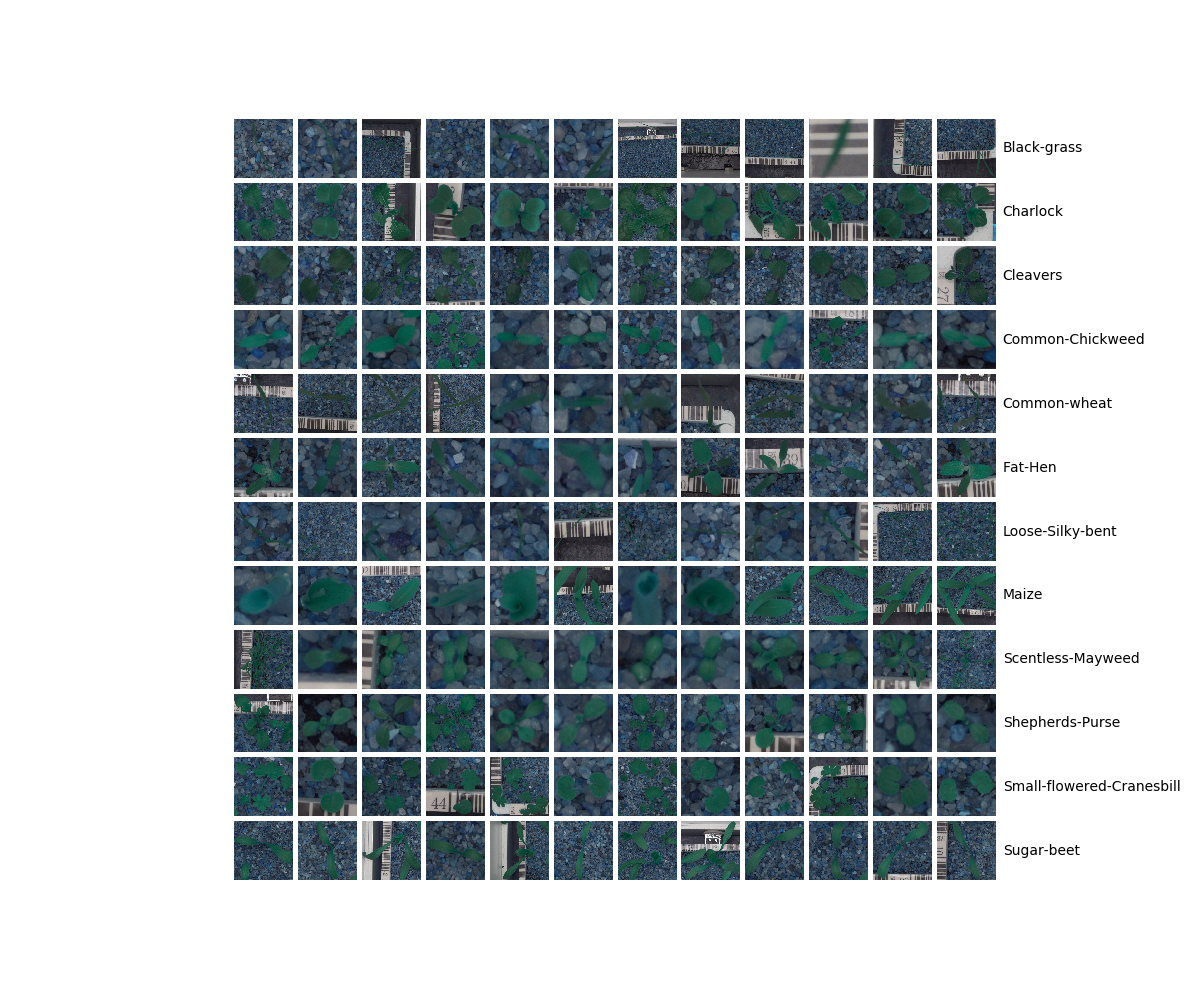
\includegraphics[width=13cm]{sample_images.png}
\caption{Plant Seedlings Dataset Samples}
\end{figure}
\end{center}

\subsection{Data manipulation}
Prior to the use of the image data for model fitting, manipulation was required to extract the features that was relevant to my analysis. Most of the data feature processing is based on python module openCV\citep{howse2013opencv} and sklearn\citep{pedregosa2011scikit}.
\begin{itemize}
\item[1)] Due to the different image sizes, we resized to a fixed size of 128 X 128.
\item[2)] Convert images to different color spaces, RGB(Red Green Blue), HSV(Hue Saturation Value), a color model based on the physiological characteristics of a person's observation of color (the human visual system is more sensitive to brightness than the color value), and HLS(Hue Saturation Lightness). 
\item[3)] Extract the histogram of the image to reduce the feature dimension
\item[4)] Based on the image features, we found that the pixel distribution is bimodal, that is, there is a big variance between the plant and the background. Through the threshold segmentation method, the image histogram is extracted after the mask.
\item[5)] During the fitting process, we separate 20\% of the dataset as test set for evaluation.
\end{itemize}


\subsection{Model evaluation metric}
Normally, for binary classification problem, the predition results will be as follows:

\begin{table}[h]
\centering
\begin{tabular}{ccc}
\hline
\diagbox{Label}{Predition} & +1 & -1 \\
\hline
+1&True Positive(TP)&False Negetive(FN)\\
-1&False Positive(FP)&True Negetive(TN)\\
\hline
\end{tabular}
\caption{Analysis of the results of the binary classification problem}
\end{table}

The metrics for classification model evaluation usually can be accuracy, precision, recall, f1-score, ROC curve, AUC, etc. Their calculation formula is as follows:
\begin{itemize}
\item[1)] Accuracy = (TP+TN)/All Samples, accuracy is the most common and basic evaluation metric. However, in the case of unbalanced positive and negative cases, especially when we are more interested in the minority class, it will have the ``accuracy paradox".
\item[2)] Precision = TP/(TP+FP) 
\item[3)] Recall = TP/(TP+FN)
\item[4)] F1-score = 2 * Precision * Recall/(Precision + Recall), F1-score is a metric that takes into account precision and recall. In the case of multi-class classification, macro-average is better than micro-average, because macro-average treats each class equally, so its value is mainly affected by rare class, and micro-average is just same as accuracy in one label classification problem.
\item[5)] True Positive Rate(TPR) = TP/(TP+FN) = TP/actual positives, False Postive Rate(FPR) = FP/(FP+TN) = FP/actual negatives, the ROC curve is composed of points (FPR, TPR) that set different thresholds, and AUC is the area of the ROC. The bigger the AUC, the better.
\end{itemize}

In this project, we comprehensively use these two types of classification model metrics to examine the image classification performance of different models.

\subsection{Computing languages}
python: use sklearn, opencv and matplotlib for machine learning, computer vision task, data analyzing and plotting.
R: for ggplot.
bash: for building the workflow.


\subsection{Model fitting}
KNN: Calculate the distance of each feature corresponding to the new data and the data in the sample set, extract the classification labels of the k most similar data, and select the classification with the most occurrences among the most similar data as the classification of the new data. One of the advantages of KNN is that the model is easy to understand and usually does not require too much adjustment to get good performance. Trying this algorithm is a good benchmark before considering the use of more advanced techniques. It is usually very fast to build a KNN model,  but if the training set is large (the number of features is large or the number of samples is large), the prediction speed may be slow. When using the KNN, it is important to preprocess the data. Although the KNN algorithm is easy to understand, it is often not used in practice because it is slow to predict and cannot process data sets with many features.
\\
\\
SVM: The mathematical principle behind the support vector machine is a bit complicated, and the main idea is to find the hyperplane with the largest classification interval.The SVM is a very powerful model that performs well on low-dimensional data and high-dimensional data, while the disadvantage of SVM is that it takes great care to preprocess data and tuning. This is why many applications today use tree-based models, such as random forests or gradient boosts, which require little pre-processing. 
\\
\\
Ensemble methods like random forests and xgboost are based on dicision tree model, they use the methods of bagging and boosting respectively. Their advantage is that they can get a good training result with almost no data pre-processing and reduce over-fitting through multiple weak learning models. 



\section{Results}
\subsection{Data manipulation}
As we can see from the histogram below, it has obvious bottom-breaking crests, which we can explain from the images, the background of the images is mostly stone and completely different from green plants, which makes it possible to mask out the plants according to different image digital number threshold (Figure3).
\begin{center}
\begin{figure}[htb]
\centering 
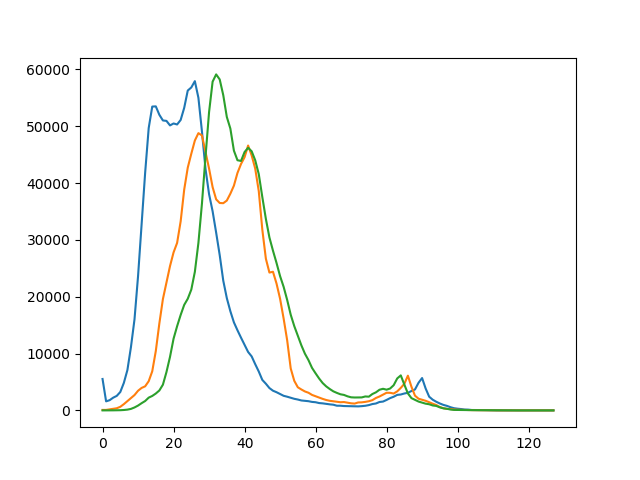
\includegraphics[width=8cm]{historgram.png}
\caption{RGB Channels Histogram Distribution}
\end{figure}
\end{center}
Finally, we select the digital number data of the three color spaces, the data after calculating the histogram, and the data after masking and histogram dimensionality reduction. According to the statistics of 4750 images, we can see that raw pixel images will occupies 228.00MB memory, while after calculating the histogram, it takes only 14.25MB, which is 16 times smaller than raw pixels data.
\begin{center}
\begin{figure}[htb]
\centering 
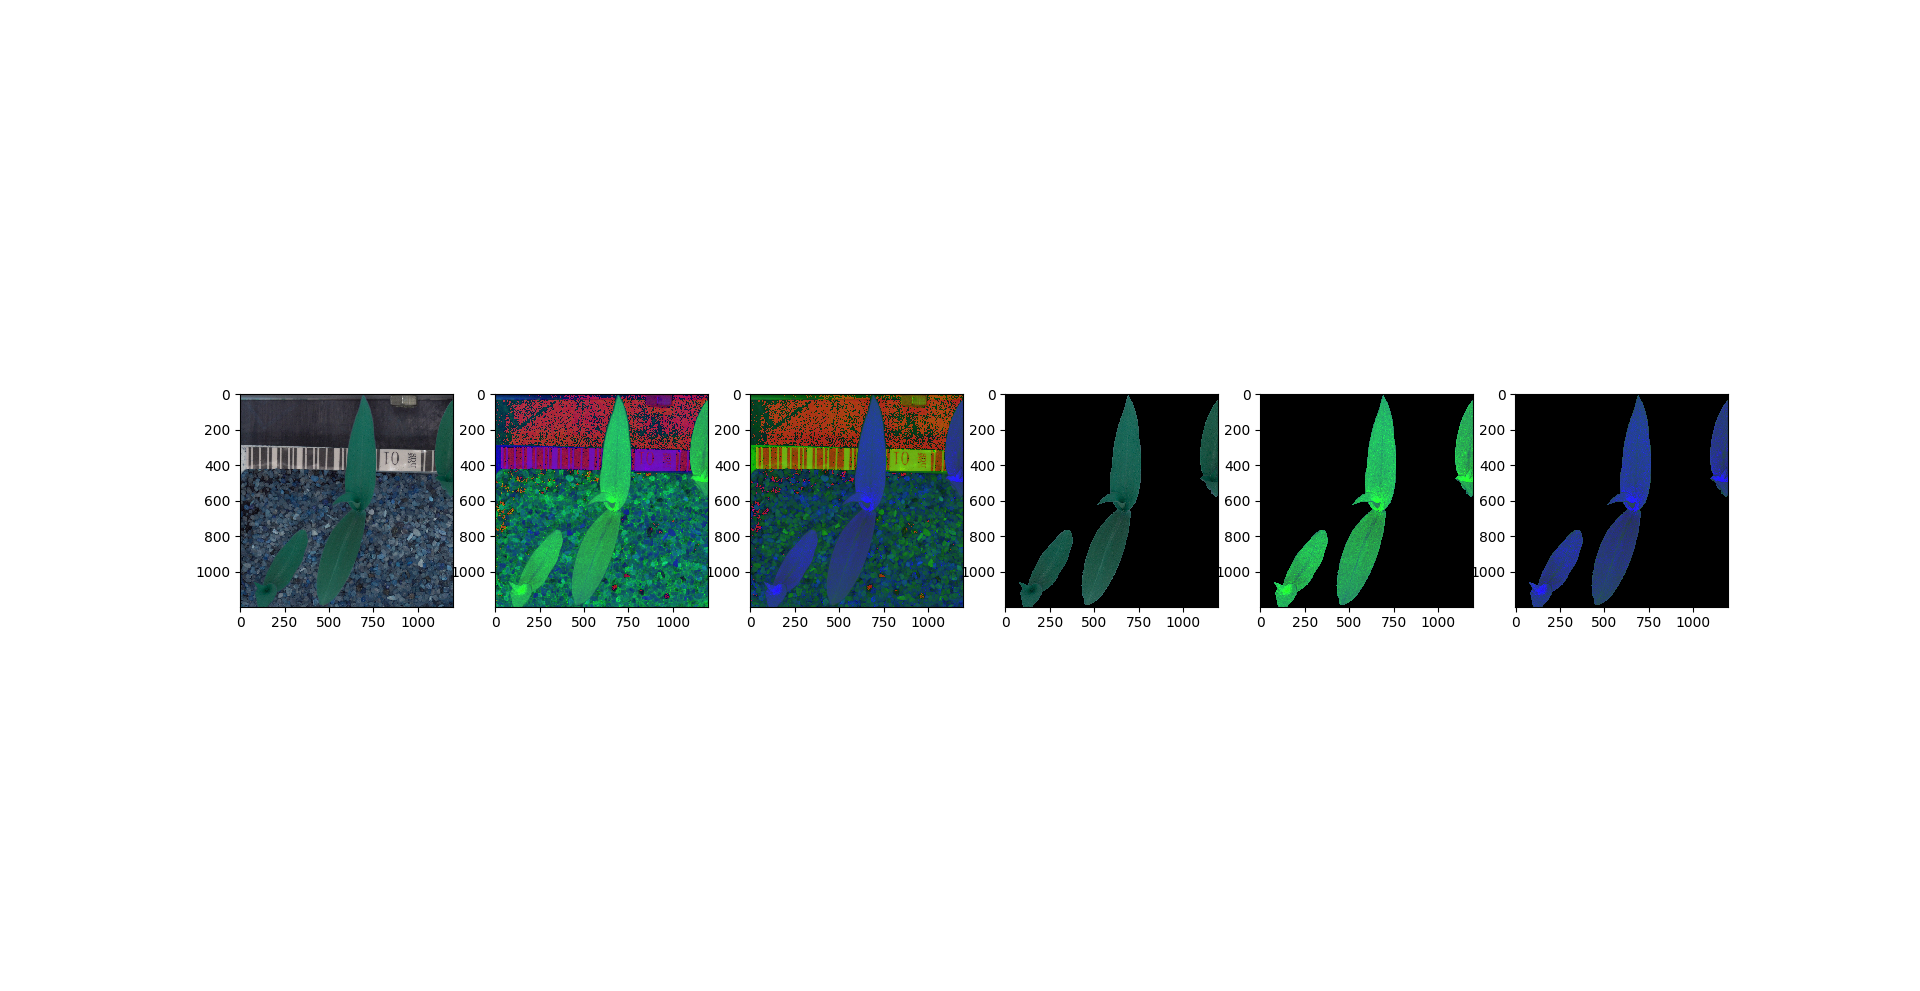
\includegraphics[trim = 50mm 80mm 00mm 80mm, clip=true, width=15cm]{preprocess_images.png}
\caption{Image after color space conversion and masking}
Images from left to right are BGR, HSV HLS color spaces.
\end{figure}
\end{center}

\subsection{KNN model comparison}
KNN is the one of the simplest and most efficient algorithm for classification model. Generally, KNN has two important hyperparameter, the number of nearest neighbors and the metrics for distances between data points, here I search for the hyperparameter K based on HSV color space after masking and histogram calculation for 1 to 20 (Figure4). 
\begin{center}
\begin{figure}[htb]
\centering 
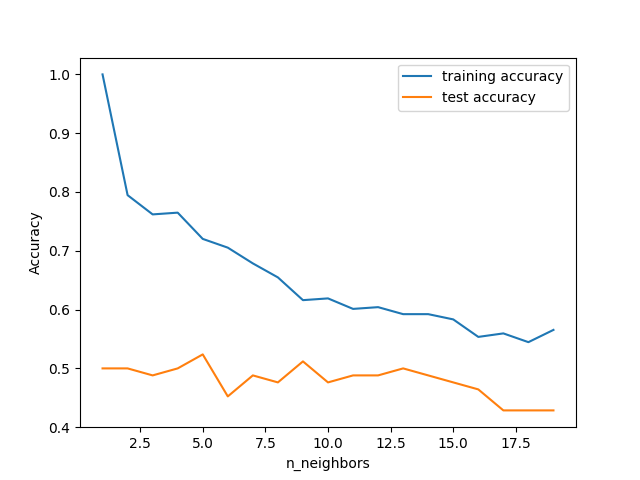
\includegraphics[width=8cm]{find_hyperparameterK.png}
\caption{RGB Channels Histogram Distribution}
\end{figure}
\end{center}
Result shows that when considering only one single neighbor, the predition on the training set are perfect, and as the number of neighbors increase, the model becomes simpler and the accuracy decreases. The test set accuracy for single neighbor is lower than when using more neighbors, which means that the model of a single neighbor is too complex, lead to overfitting, so the best number should be when the two urves are relatively close, and her I chose K=9 to further explore different data processing methods.

\begin{table}[htb]
\centering
\resizebox{\textwidth}{!}{
\begin{tabular}{cccccccccc}
\hline
\diagbox{ACC/Time}{Model} &RGB&HSV&HSL&histoRGB&histoHSV&histoHSL&maskRGB&maskHSV&maskHSL\\
\hline
Training set(\%)&41.68&49.61&51.53&70.58&76.79&77.11&74.55&78.39&78.32\\
Test set(\%)&26.42&38.53&38.53&58.84&67.16&70.84&68.21&72.42&71.37\\
Time consuming(s)&19'47&19'57&19'55&10&6&6&2&2&2\\
\hline
\end{tabular}}
\caption{KNN model comparison}
\end{table}

\begin{center}
\begin{figure}[htb]
\centering 
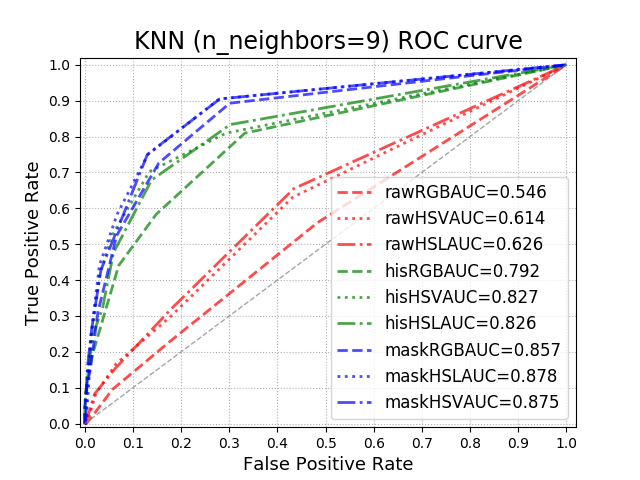
\includegraphics[width=8cm]{KNN-ROC.png}
\caption{KNN models ROC curve}
\end{figure}
\end{center} 
So by combining the three color spaces with the three processing methods, we have fitted the KNN algorithm to the 9 different image processing data. Using ROC curve and the area under the curve (AUC) as evaluation metric, we can find that:
\begin{itemize}
\item[1)] KNN model fitting performance on histogram data is generally better than raw image pixel data, and spend expected less time.
\item[2)] Model performance better on HSV, HLS color space than RGB, but silghtly different between them.
\item[3)] Whether masking or not does not have much effect on the results.
\end{itemize}

    
\subsection{KNN, SVM, Random Forest and XGBoot model comparison}
Based on the fitting results of KNN in different image processing methods, I choose the HSV color space mask data as object, compared the fittig results of these several models. Although Gridsearch was used to find the best hyperparameter for the Random Forest, it seems to play a minor role in this task, so for the SVM and the ensemble models, I mainly use sklearn's default parameters in order to build a basline model as soon as possible. And the result shows as below:
\begin{center}
\begin{figure}[htb]
\centering 
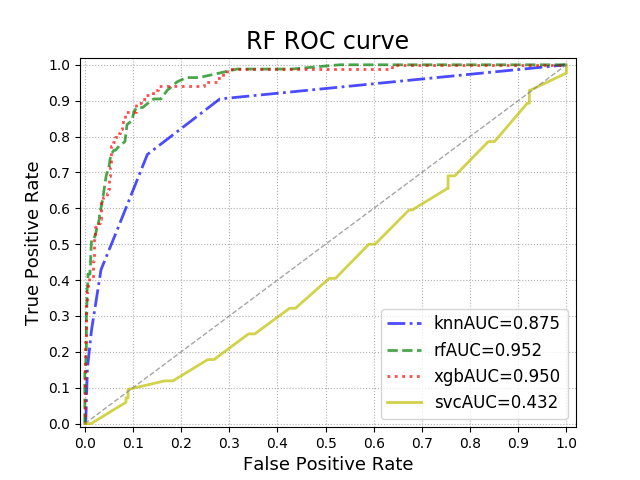
\includegraphics[width=8cm]{All-ROC.png}
\caption{KNN, SVM, Random Forest and XGBoot ROC Curve}
\end{figure}
\end{center}

\begin{table}[h]
\centering
\resizebox{\textwidth}{!}{
\begin{tabular}{ccccc}
\hline
\diagbox{Metrics}{Model} &KNN&SVM&Random Forest&XGBoost\\
\hline
Accuracy&72.42&13.16&85.58&87.58\\
AUC&0.953&0.606&0.985&0.988\\
Micro F1 score&0.72&0.13&0.86&0.88\\
Macro F1 score&0.70&0.02&0.85&0.86\\
Time consuming(s)&2&1'5&2&2'36\\
\hline
\end{tabular}}
\caption{Four models comparison}
\end{table}

As you can see from the results, although the SVM can achieve the same accuracy as the ensemble methods (99\%), its generalization ability is much worse, only 13.16\% accuracy. As for the other three models, we can say that XGBoost performs the best, followed by the Random Forest, finally the KNN. 
    
\subsection{ResNets18 and transfer learning}
Based on Pytorch's deep learning framework, the parameters are fine-turn from scratch, or freeze all layers, and add a fully connected layer at the end for parameter optimization. And it turns out that the learning from scratch has the 95.5\% accuracy for validation set and 88.9\% for training set, while when ConvNet as fixed feature extractor, it only has 57.5\% accuracy for training set and 71.1\% for validation set.

\section{Discussion}
Overall, the above results demonstrate that when considering all five proposed models, though they were fitted in a limited time, there is much room for improvement, we can still learn some trade-off during model selection.
\\
\\
Since we are dealing with unstructured data, it is hard to judge and extract the important features. In the process of applying traditional machine learning algorithms, it is very necessary to rely on the prior knowledge of the data for feature engineering. In this example, we can see this very obviously. After histogram calculation, not only can we reduce the data by 16 times but we can also improve the accuracy of 20-30\% on the KNN model. However, the performance of the model seems to be lower than I expected after masking. A reasonable explanation is that after the dimensionality reduction by the histogram calculation the noise of the background is not significantly different among different species, which is not enough to be a feature to imporve the performance of the model. And this raises another interesting issue, the machine learning algorithm usually does not care about the spatial relationship of pixels in the process of fitting image data, while convolutional neural networks can obtain some spatial information from the images through the way of weight sharing.  
\\
\\
We can also see that most of the fitting results have been overfitting due to some consensus reasons, like too much noise, insufficent training data, overly complex model etc. The image in the dataset is not uniform, the size is inconsistent and have large variance, sometimes there are more than one plant in a picture. So, it can be better if there is a better way to normalized the data. Besides, ensemble method like Random Forest and XGBoost can theoretically reduce the complexity of the model to avoid overfitting, but it goes up to 99\% accuracy for the training set, probably need more effort on hyperparameter turning.



\bibliography{Report}
\end{document}
